\FloatBarrier
\section{Retained experimental figures}\label{supp:retained-figures}
The figures in this section restore the original A19 and earlier A20 result displays. Their inputs, solver variants, calibration families and timing ledgers remain those of the retained studies. They provide the detailed evidence underlying the retained-study summaries; their samples and CPU measurements are kept separate from the retained 2,680-episode R4 study. Each original vector PDF is included without changing its plotted data.

\begin{figure}[!htbp]\centering
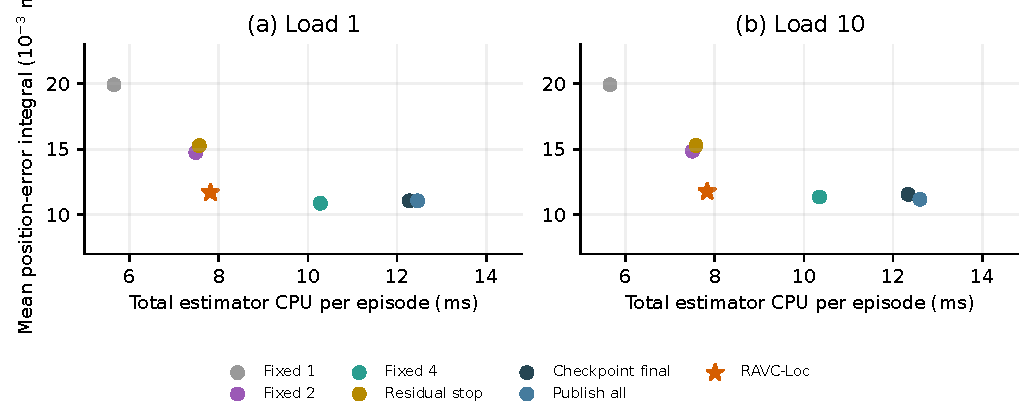
\includegraphics[width=.97\linewidth]{episode_frontier.pdf}
\caption{Retained A20 confirmation work--exposure trade-offs at load factors 1 and 10. Each point averages the same 240 independent episodes; the star marks the policy selected using the separate retained calibration set. Positions are descriptive operating points under the original estimator CPU ledger.}\label{supp:legacy-frontier}
\end{figure}
\begin{figure}[!htbp]\centering
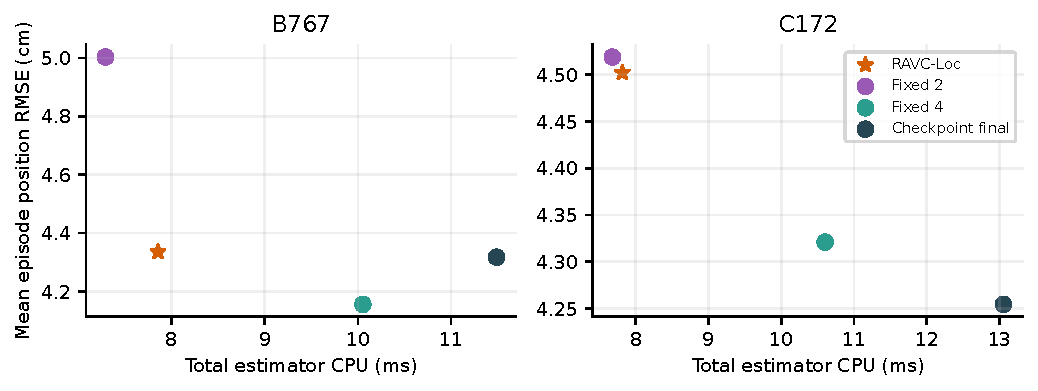
\includegraphics[width=.97\linewidth]{geometry_tradeoff.pdf}
\caption{Retained A20 confirmation trade-offs separated by aircraft geometry at load 10. The common retained calibration mixture determines the selected policy. Aircraft subgroups are descriptive and were not used for reselection.}\label{supp:legacy-geometry}
\end{figure}
\FloatBarrier
\begin{figure}[!htbp]\centering
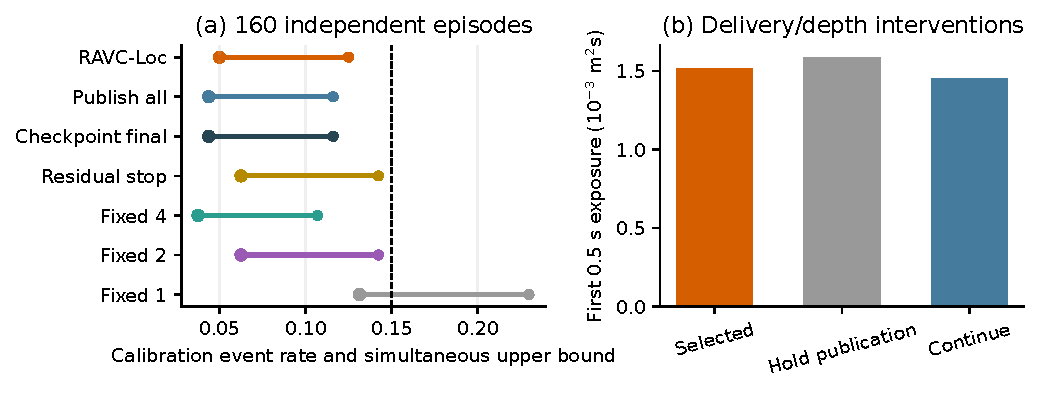
\includegraphics[width=.97\linewidth]{risk_and_delivery.pdf}
\caption{Retained A20 calibration and publication interventions. (a) Point event rates and simultaneous upper bounds for selected controls and RAVC-Loc on 160 independent calibration episodes; the dashed line is $\delta=0.15$. (b) Startup exposure on 240 confirmation episodes at load 10. Holding publication preserves stopping and the final candidate; continuation preserves publication logic and changes iteration depth.}\label{supp:legacy-risk-delivery}
\end{figure}
\begin{figure}[!htbp]\centering
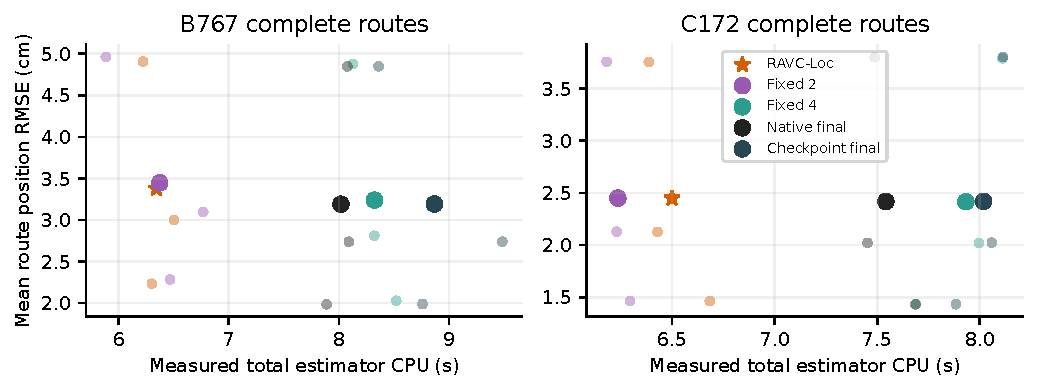
\includegraphics[width=.97\linewidth]{route_tradeoff.pdf}
\caption{Retained A20 complete-route work--error outcomes. Small points are the three retained realizations per aircraft; large points are their method means over 1,980-s routes. Every control uses the same scan cadence and delivery model within this retained block. The original total estimator CPU ledger is preserved.}\label{supp:legacy-route-tradeoff}
\end{figure}
\begin{figure}[!htbp]\centering
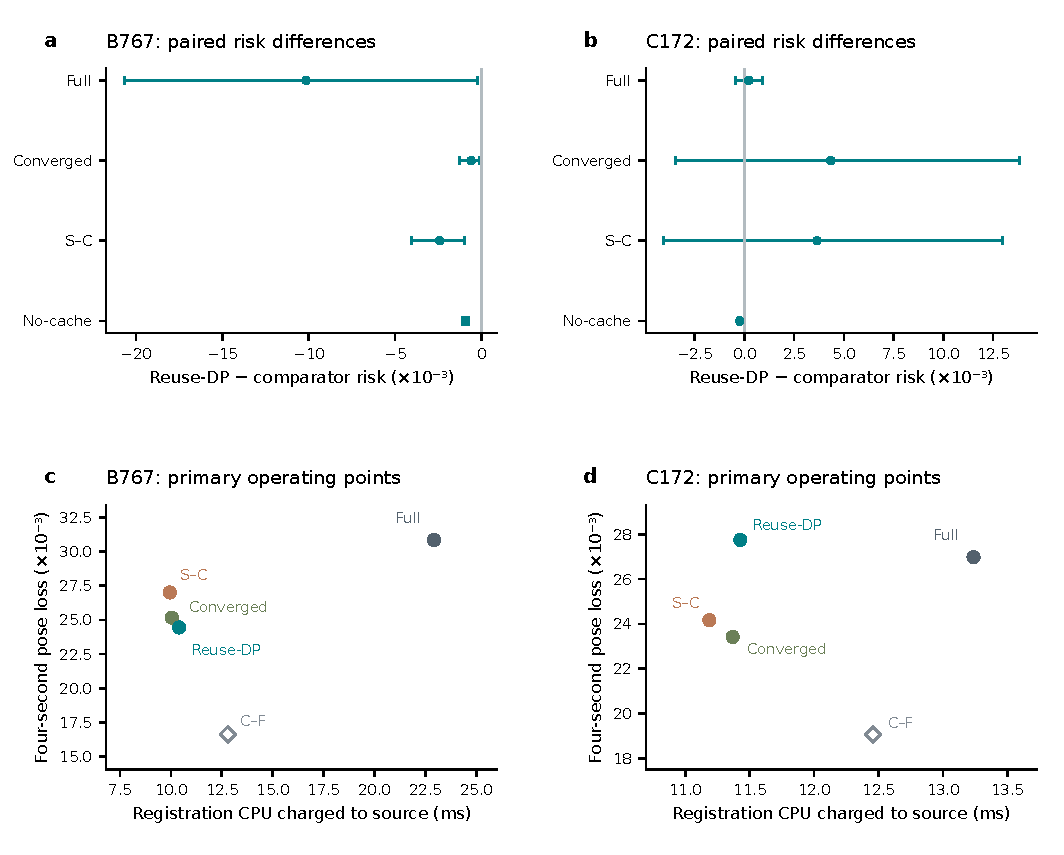
\includegraphics[width=.97\linewidth]{legacy_sources.pdf}
\caption{Retained A19 source-level controls on 240 fresh sources per aircraft at $\lambda=0.3$ and the original primary budget. (a,b) Paired differences in priced risk, Reuse-DP minus the indicated comparator, with pointwise 95\% percentile intervals from 4,000 source-bootstrap resamples. (c,d) Mean geometric loss and measured or replay-charged registration CPU. Filled markers indicate feasibility on all observed primary-budget paths; open diamonds mark the relaxed Converged--Full cascade. These action and reuse controls precede the current checkpoint family.}\label{supp:legacy-sources}
\end{figure}
\begin{figure}[!htbp]\centering
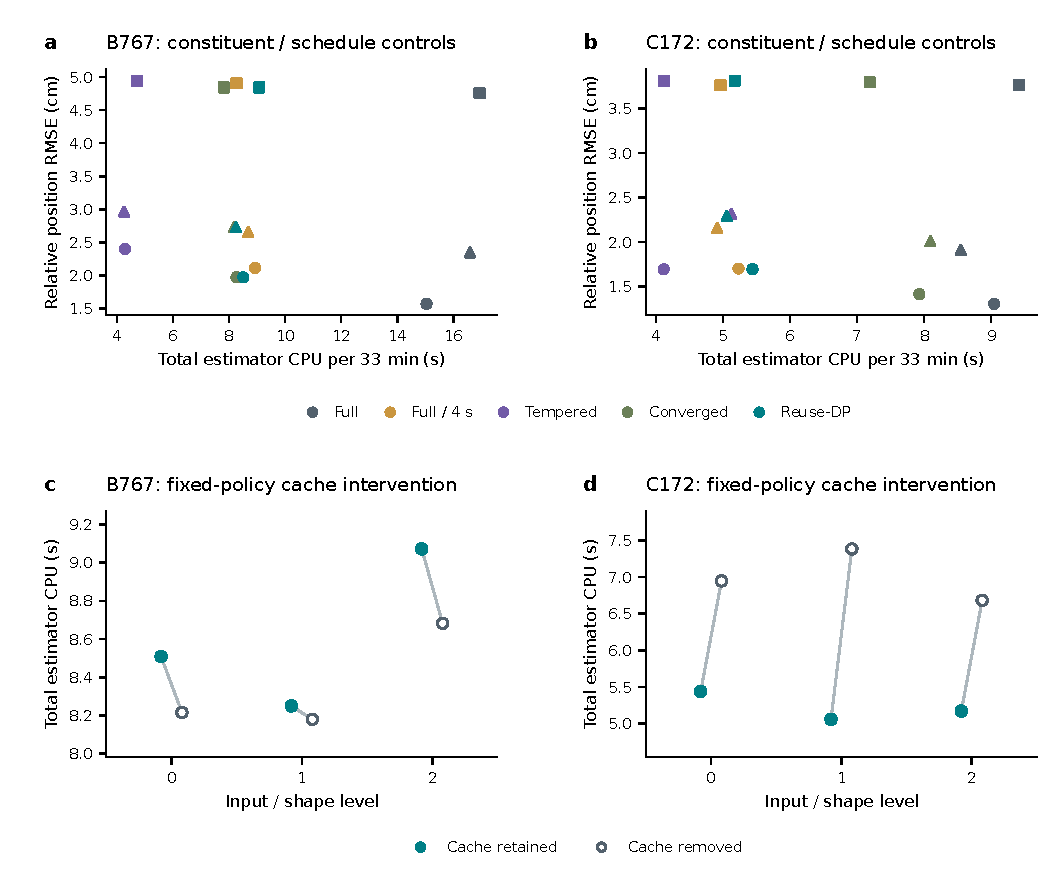
\includegraphics[width=.97\linewidth]{legacy_missions.pdf}
\caption{Retained A19 33-minute route controls and cache interventions. Upper panels compare constituent actions and schedules; lower panels remove reuse at fixed policy across the original input/shape levels. The source archive retains all realizations and the separate route CPU accounting.}\label{supp:legacy-missions}
\end{figure}
\FloatBarrier
\section{Additional physical-platform views}\label{supp:hardware}
Two further original project photographs show platform integration and the aircraft underside. The main R8 paper now includes all four original photographs; these two earlier detail layouts remain for historical continuity. The reproduction bundle preserves the four original JPEGs with their initial dimensions and byte hashes. Photographs provide qualitative engineering context; numerical localization outcomes come from the separately specified simulation inputs.
\begin{figure}[!htbp]\centering
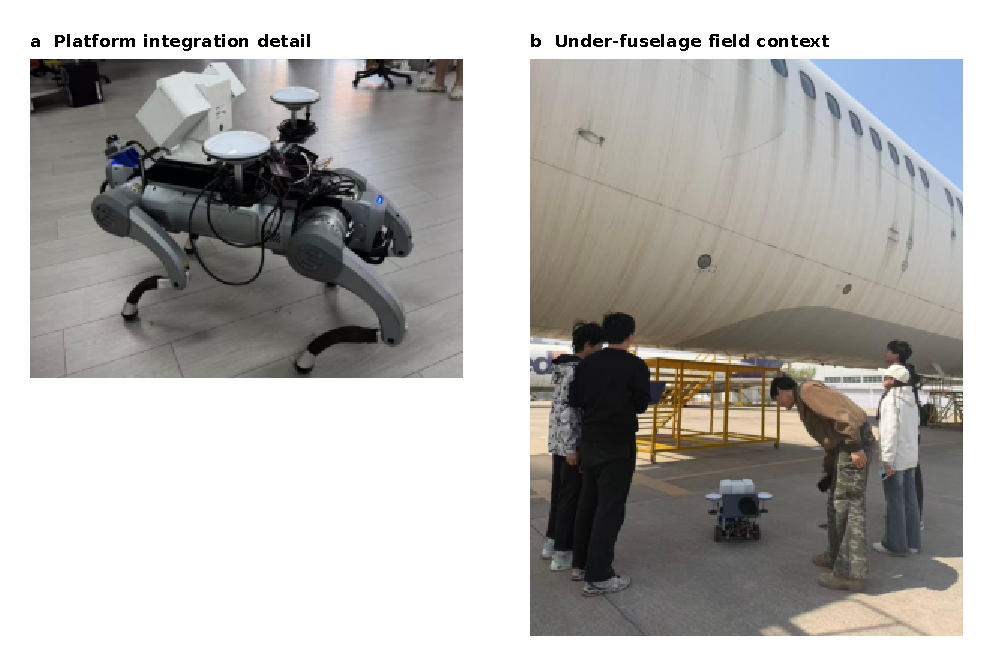
\includegraphics[width=\linewidth]{r7/hardware_details.pdf}
\caption{Additional original physical-platform photographs. (a) Side view of platform integration. (b) Field context beneath the aircraft fuselage. Both images retain their original aspect ratios without cropping, pixel retouching, contrast adjustment or generated content.}\label{supp:hardware-details}
\end{figure}
\FloatBarrier
